\documentclass[11pt,a4paper]{article}

\usepackage[margin=2.5cm]{geometry}
\usepackage{booktabs}
\usepackage{longtable}
\usepackage{array}
\usepackage{graphicx}
\usepackage{xcolor}
\usepackage{tikz}
\usetikzlibrary{positioning,arrows.meta,fit,backgrounds}
\usepackage{hyperref}
\usepackage{parskip}
\usepackage{fancyhdr}
\usepackage{titlesec}
\usepackage{enumitem}

\definecolor{okgreen}{HTML}{3F8A6F}
\definecolor{blockedred}{HTML}{B8503A}
\definecolor{sensorgold}{HTML}{C9A227}
\definecolor{pendinggrey}{HTML}{8A8371}
\definecolor{nagrey}{HTML}{948C78}
\definecolor{accentblue}{HTML}{5C7A99}
\definecolor{headergrey}{HTML}{333333}

\titleformat{\section}{\large\bfseries\color{headergrey}}{\thesection}{0.6em}{}
\titleformat{\subsection}{\normalsize\bfseries\color{headergrey}}{\thesubsection}{0.6em}{}

\hypersetup{
  colorlinks=true,
  linkcolor=accentblue,
  urlcolor=accentblue,
  citecolor=accentblue,
  pdftitle={Native Isaac ROS on Jetson Orin Nano / JetPack 7},
  pdfauthor={perseus-lite project}
}

\pagestyle{fancy}
\fancyhf{}
\fancyhead[L]{\small\textcolor{headergrey}{Native Isaac ROS on Orin Nano / JetPack 7}}
\fancyhead[R]{\small\textcolor{headergrey}{\thepage}}
\renewcommand{\headrulewidth}{0.4pt}

\newcommand{\statuschip}[2]{%
  \tikz[baseline=-0.6ex]\node[fill=#1,text=white,rounded corners=2pt,inner sep=2pt,font=\scriptsize\bfseries]{#2};%
}

\begin{document}

% ---------------------------------------------------------------------
% Title page
% ---------------------------------------------------------------------
\begin{titlepage}
\centering
\vspace*{2.5cm}
{\Huge\bfseries Native Isaac ROS on Jetson Orin Nano\par}
\vspace{0.4cm}
{\Large A From-Source Build Report for JetPack 7\par}
\vspace{1.5cm}
{\large \texttt{perseus-lite} project --- \texttt{feature/isaac-ros-nitros-source-build}\par}
\vspace{0.3cm}
{\large \today\par}
\vspace{2cm}

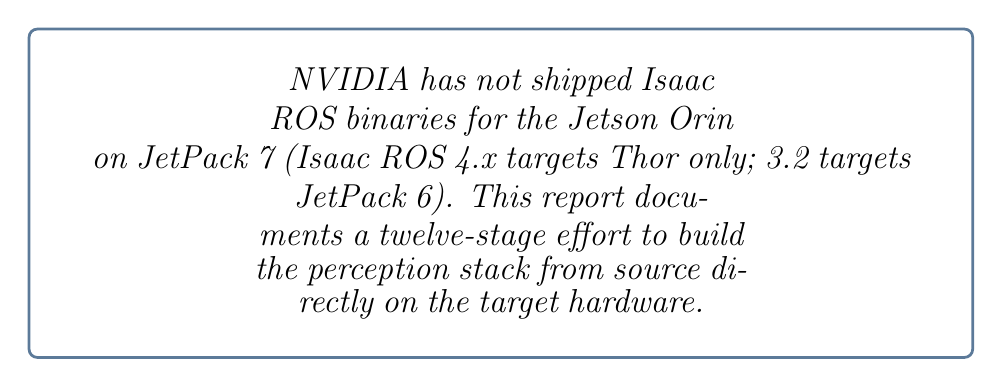
\begin{tikzpicture}
  \node[draw=accentblue, line width=1pt, rounded corners=3pt, inner sep=14pt, text width=11cm, align=center]
    {\large\itshape
     NVIDIA has not shipped Isaac ROS binaries for the Jetson Orin\\
     on JetPack 7 (Isaac ROS 4.x targets Thor only; 3.2 targets\\
     JetPack 6). This report documents a twelve-stage effort to build\\
     the perception stack from source directly on the target hardware.};
\end{tikzpicture}

\vfill

\begin{minipage}{0.85\textwidth}
\centering
\small
\textbf{Summary of outcome:} of the 29 relevant Isaac ROS GEM repositories surveyed,
\textbf{7 were built and verified working natively}, \textbf{3 were built successfully
but are blocked at runtime} by fully root-caused hardware or platform limits
(none are code defects), and the remainder are either sensor-gated, architecturally
inapplicable to this robot, or not yet attempted.
\end{minipage}

\vspace{1cm}
\end{titlepage}

\tableofcontents
\newpage

% ---------------------------------------------------------------------
\section{Executive Summary}

This report documents an effort to build NVIDIA's Isaac ROS GPU-accelerated
perception stack \emph{entirely from source}, running natively (no containers)
on a Jetson Orin Nano under JetPack~7 --- a hardware/software combination NVIDIA
does not yet officially support. The work proceeded as twelve incremental
stages, each with its own build, integration, and verification pass against
either NVIDIA's own test fixtures or, where possible, real recorded sensor data.

Seven perception capabilities are now verified working natively: AprilTag
fiducial detection, generic TensorRT DNN inference, YOLOv8 object detection,
U-Net semantic segmentation, CenterPose monocular 3D pose estimation, an
occupancy-grid GPU lidar localizer, and a ten-node composability test proving
several of the above can run concurrently in a single process without
interference. Three further capabilities were fully built --- including, in
two cases, genuine custom CUDA kernel compilation --- but are blocked at
runtime by causes outside the scope of a source rebuild: a CPU instruction-set
mismatch in a closed-source vendor binary, absent encoder silicon on this
particular Jetson SKU, and a small, boot-configured GPU memory carveout.
Each blocker is root-caused in full rather than left as an unexplained failure.

\begin{figure}[h]
\centering
\includegraphics[width=0.92\textwidth]{stage_status.pdf}
\caption{Outcome of all twelve stages. A blocked stage means the build succeeded but a runtime limitation, root-caused in Section~\ref{sec:blockers}, prevents the capability from running end to end.}
\end{figure}

% ---------------------------------------------------------------------
\section{Background and Motivation}

The \texttt{perseus-lite} robot's Jetson Orin Nano runs JetPack~7
(L4T~R39.2.0, CUDA~13.2, Ubuntu~24.04). NVIDIA's Isaac ROS GPU perception
stack, which the robot's Jetson-based vision pipeline depends on for
NITROS zero-copy message transport and TensorRT-accelerated inference,
ships as prebuilt binaries for only two configurations: Isaac ROS~3.2
(JetPack~6.x) and Isaac ROS~4.x (Thor only). Neither covers this robot's
actual hardware. NVIDIA staff have confirmed JetPack~7 support for Orin
is planned but undated.

Rather than wait, this project attempted to close the gap by building the
relevant Isaac ROS packages from source, directly against the installed
CUDA~13.2/JetPack~7 toolchain, and verifying each capability with the same
rigor NVIDIA's own test suites use --- reusing their published test fixtures,
ground-truth values, and tolerances wherever available, rather than
inventing new pass/fail criteria.

A companion, separate effort in the same repository (\texttt{software/docker/\allowbreak
isaac-ros/}) runs the officially supported JetPack~6 image inside Docker.
This report concerns only the from-source, native track.

% ---------------------------------------------------------------------
\section{Methodology}

Each stage followed the same discipline:

\begin{enumerate}[leftmargin=1.4cm]
\item \textbf{Clone} the relevant NVIDIA GitHub repository into a
  gitignored working directory --- nothing from NVIDIA's source trees is
  committed to the project repository, only our own build scripts and
  documentation referencing them (a licensing requirement of NVIDIA's
  source-available Isaac ROS terms).
\item \textbf{Build} with an explicit toolchain: \texttt{CUDACXX} pointed
  at the CUDA~13.2 \texttt{nvcc}, and \texttt{-DCMAKE\_CUDA\_ARCHITECTURES=87}
  set explicitly for Orin's real Ampere streaming-multiprocessor
  architecture, since CMake's own auto-detection runs before Isaac ROS's
  fallback logic and fails on a fresh configure otherwise.
\item \textbf{Wire} a minimal launch graph directly instantiating the
  needed composable nodes --- not NVIDIA's higher-level launch-file
  wrappers, whose ROS parameter names for topics do not always match the
  node's actual hardcoded wire topic (a mismatch discovered and documented
  in Stage~5).
\item \textbf{Verify} against a real signal wherever NVIDIA supplies one:
  a pixel-exact match to a ground-truth image (Stage~4), a numerically
  correct 3D pose against a real trained model and measured ground truth
  (Stage~8), or a recovered lidar pose within NVIDIA's own test tolerance
  against real recorded sensor data (Stage~12). Where NVIDIA's fixture uses
  randomly-initialized weights, verification is scoped to structural
  correctness of the message, matching NVIDIA's own test scope for the
  same fixture.
\item \textbf{Document} the outcome unconditionally --- successes,
  failures, and root-caused blockers all receive the same level of
  detail, including exact reproduction commands.
\end{enumerate}

% ---------------------------------------------------------------------
\section{System Architecture}

\subsection{The NITROS composable-node pattern}

Every DNN-based capability (Stages 5, 5-follow-up, 7, 8, 11) shares the
same three-stage composable-node chain: an image encoder resizes and
normalizes an incoming image into a tensor, a TensorRT node runs
inference, and a capability-specific decoder converts raw tensor output
into a typed ROS message (detections, a segmentation mask, a 3D pose).
Figure~\ref{fig:pipeline} shows this pattern, plus Stage~10's extension
of it: four such pipelines, each given its own ROS namespace, composed
into a single shared process to prove they do not interfere with one
another.

\begin{figure}[h]
\centering
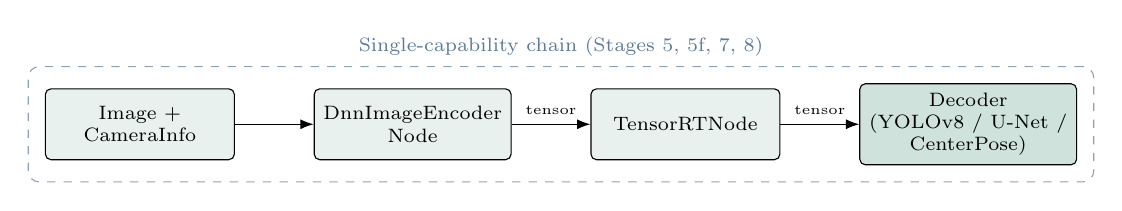
\begin{tikzpicture}[
  node distance=6mm and 10mm,
  block/.style={draw, rounded corners=2pt, minimum height=9mm, minimum width=24mm, align=center, font=\scriptsize, fill=white},
  pipeline/.style={draw=accentblue!70, dashed, rounded corners=4pt, inner sep=6pt},
  lbl/.style={font=\scriptsize\itshape, text=headergrey}
]
  % single pipeline exemplar
  \node[block, fill=okgreen!12] (img) {Image +\\CameraInfo};
  \node[block, right=of img, fill=okgreen!12] (enc) {DnnImageEncoder\\Node};
  \node[block, right=of enc, fill=okgreen!12] (trt) {TensorRTNode};
  \node[block, right=of trt, fill=okgreen!25] (dec) {Decoder\\(YOLOv8 / U-Net /\\CenterPose)};

  \draw[-Latex] (img) -- (enc);
  \draw[-Latex] (enc) -- node[above,font=\tiny]{tensor} (trt);
  \draw[-Latex] (trt) -- node[above,font=\tiny]{tensor} (dec);

  \node[pipeline, fit=(img)(enc)(trt)(dec), label={[font=\scriptsize,text=accentblue]above:Single-capability chain (Stages 5, 5f, 7, 8)}] (p1) {};

\end{tikzpicture}
\vspace{4mm}

\begin{tikzpicture}[
  node distance=3mm and 6mm,
  smallblock/.style={draw, rounded corners=1.5pt, minimum height=6mm, minimum width=18mm, align=center, font=\tiny, fill=white},
  nsbox/.style={draw=accentblue!60, rounded corners=3pt, inner sep=4pt, fill=accentblue!4},
  pipeline/.style={draw=accentblue!70, dashed, rounded corners=4pt, inner sep=6pt},
  lbl/.style={font=\scriptsize\bfseries, text=accentblue}
]
  \node[nsbox] (ns1) {
    \begin{tikzpicture}[node distance=2mm]
      \node[smallblock] (a1) {AprilTagNode};
    \end{tikzpicture}
  };
  \node[lbl, above=0 of ns1] {/apriltag};

  \node[nsbox, right=8mm of ns1] (ns2) {
    \begin{tikzpicture}[node distance=2mm]
      \node[smallblock] (b1) {Encoder};
      \node[smallblock, right=2mm of b1] (b2) {TensorRT};
      \node[smallblock, right=2mm of b2] (b3) {YOLOv8\\Decoder};
      \draw[-Latex,thin] (b1)--(b2); \draw[-Latex,thin] (b2)--(b3);
    \end{tikzpicture}
  };
  \node[lbl, above=0 of ns2] {/yolov8};

  \node[nsbox, below=6mm of ns1, xshift=0mm] (ns3) {
    \begin{tikzpicture}[node distance=2mm]
      \node[smallblock] (c1) {Encoder};
      \node[smallblock, right=2mm of c1] (c2) {TensorRT};
      \node[smallblock, right=2mm of c2] (c3) {U-Net\\Decoder};
      \draw[-Latex,thin] (c1)--(c2); \draw[-Latex,thin] (c2)--(c3);
    \end{tikzpicture}
  };
  \node[lbl, above=0 of ns3] {/unet};

  \node[nsbox, right=8mm of ns3] (ns4) {
    \begin{tikzpicture}[node distance=2mm]
      \node[smallblock] (d1) {Encoder};
      \node[smallblock, right=2mm of d1] (d2) {TensorRT};
      \node[smallblock, right=2mm of d2] (d3) {CenterPose\\Decoder};
      \draw[-Latex,thin] (d1)--(d2); \draw[-Latex,thin] (d2)--(d3);
    \end{tikzpicture}
  };
  \node[lbl, above=0 of ns4] {/centerpose};

  \begin{scope}[on background layer]
    \node[pipeline, fit=(ns1)(ns2)(ns3)(ns4), inner sep=10pt,
          label={[font=\scriptsize,text=accentblue]above:\texttt{combined\_pipeline\_container} -- one process, one GPU context (Stage 10)}] {};
  \end{scope}
\end{tikzpicture}
\caption{The shared encoder/TensorRT/decoder pattern (top), and Stage~10's
  composition of four such namespaced pipelines into one shared process
  (bottom) --- verified to run concurrently without topic collisions or
  resource contention.}
\label{fig:pipeline}
\end{figure}

Namespacing matters here for a concrete reason: every encoder node
publishes to the literal hardcoded topic \texttt{tensors}, and every
\texttt{TensorRTNode} subscribes to \texttt{tensor\_pub} regardless of
which model it is running. Without a distinct ROS namespace per pipeline,
three simultaneous encoder/TensorRT chains would collide directly on
these relative topic names.

% ---------------------------------------------------------------------
\section{Results by Stage}

Table~\ref{tab:stages} summarizes all twelve stages. Full technical detail,
exact build commands, and root-cause analysis for each are maintained in
the project's own documentation
(\texttt{docs/source/systems/software/isaac-ros-nitros-source-build.md}).

\begin{longtable}{@{}p{1.0cm}p{4.6cm}p{2.1cm}p{7.0cm}@{}}
\toprule
\textbf{Stage} & \textbf{Capability} & \textbf{Outcome} & \textbf{Note} \\
\midrule
\endhead
0--1 & Environment stand-up; GXF binary compatibility check & \statuschip{okgreen}{VERIFIED} &
  Confirmed NVIDIA's published SBSA GXF binaries load on Orin --- the key decision gate that avoided a much larger from-scratch GXF rebuild. \\
2--3 & NITROS core build & \statuschip{okgreen}{VERIFIED} &
  Minimal round-trip proof-of-life for the zero-copy message transport layer. \\
4 & AprilTag fiducial detection & \statuschip{okgreen}{VERIFIED} &
  Pixel-exact match against NVIDIA's ground-truth fixture; live-camera pipeline running at steady 10\,Hz. \\
5 & Generic DNN inference (TensorRT) & \statuschip{okgreen}{VERIFIED} &
  Full image$\to$resize/normalize$\to$MobileNetV2 classification round trip; exact $[1,1000]$ output. \\
5f & YOLOv8 object detection & \statuschip{okgreen}{VERIFIED} &
  Full encode$\to$infer$\to$decode chain; structurally valid detections (random-weight test fixture). \\
6 & Visual SLAM (cuVSLAM) & \statuschip{blockedred}{BLOCKED} &
  Builds clean; NVIDIA's published binary requires SVE2, an ARM instruction-set extension Orin's CPU does not implement. Upstream binary defect, not fixable locally. \\
7 & U-Net semantic segmentation & \statuschip{okgreen}{VERIFIED} &
  960$\times$544 raw and colorized masks, correct shapes and encodings. \\
8 & CenterPose monocular 3D pose & \statuschip{okgreen}{VERIFIED} &
  \textbf{Strongest result in the series}: real trained model, 2/2 detections matching NVIDIA's measured ground truth, depths within 0.5\,m. \\
9 & Hardware H.264 codec & \statuschip{blockedred}{BLOCKED} &
  Builds clean; this Jetson Orin \emph{Nano} SKU has no hardware video encoder silicon at all. Decode reaches the driver layer before failing in a closed-source buffer-mapping call. \\
10 & Combined multi-pipeline composability & \statuschip{okgreen}{VERIFIED} &
  AprilTag, YOLOv8, U-Net, and CenterPose running concurrently in one process with no interference. \\
11 & ESS deep stereo depth & \statuschip{blockedred}{BLOCKED} &
  Builds clean, including a genuine custom CUDA kernel. Runtime blocked by exhaustion of Tegra's small, boot-configured CMA memory carveout --- not general system RAM. \\
12 & Occupancy-grid lidar localizer & \statuschip{okgreen}{VERIFIED} &
  First capability matched to the robot's 2D lidar rather than its camera; GPU scan-matching recovered a pose matching NVIDIA's recorded ground truth. \\
\bottomrule
\caption{Outcome of all twelve build stages.}
\label{tab:stages}
\end{longtable}

% ---------------------------------------------------------------------
\section{Root-Caused Blockers}
\label{sec:blockers}

Three stages built successfully but are blocked at runtime. In every case
the root cause was tracked down to a specific, external limitation rather
than left as an unexplained failure, and none required abandoning the
investigation without an answer.

\begin{longtable}{@{}p{2.6cm}p{5.6cm}p{6.4cm}@{}}
\toprule
\textbf{Stage} & \textbf{Symptom} & \textbf{Root cause} \\
\midrule
\endhead
6 --- Visual SLAM &
  Immediate \texttt{SIGILL} on library load, before any application code runs &
  NVIDIA's \texttt{aarch64\_jetpack70} cuVSLAM binary contains SVE2 instructions in its static initializer. Orin's Cortex-A78AE CPU implements NEON but not SVE at all --- confirmed via \texttt{/proc/cpuinfo} and disassembly comparison against the JetPack~6.1 binary variant, which has no SVE instructions but wants an incompatible older CUDA ABI instead. \\
\addlinespace
9 --- H.264 codec &
  Encoder fails to open its device node; decoder initializes but fails deeper in the pipeline &
  \texttt{/dev/v4l2-nvenc} does not exist on this specific Jetson Orin \emph{Nano} module (confirmed via direct device enumeration) --- only the Orin NX and AGX variants include the hardware encoder engine. Decode reaches NVIDIA's closed-source \texttt{libnvbufsurface} before failing with an unsupported-platform error. \\
\addlinespace
11 --- Stereo depth &
  \texttt{cudaErrorMemoryAllocation} despite gigabytes of free system RAM &
  Tegra's CMA (contiguous memory allocator) carveout is a small, boot-time-configured memory pool (256\,MB total on this device) entirely separate from ordinary RAM, used for GPU/ISP buffer sharing. The desktop compositor alone was found to consume nearly all of it, leaving too little headroom for this stage's fifteen-node stereo pipeline. Resolvable only by a system boot-configuration change, which was intentionally left for a deliberate decision rather than made unilaterally. \\
\bottomrule
\caption{Root cause of every blocked stage.}
\end{longtable}

% ---------------------------------------------------------------------
\section{The Full Isaac ROS Catalog in Context}

NVIDIA's Isaac ROS ships as roughly 29 independent GEM (GPU-accelerated
robotics capability) repositories. Figure~\ref{fig:map} places this
project's twelve stages against the full catalog. A large share of the
untouched remainder is not actually available work: seven repositories
target hardware this robot does not have at an architectural level
(NVIDIA's Nova reference platform, CSI camera frameworks, a humanoid
robot's specific packages), and three more require a depth or stereo
camera the robot does not carry.

\begin{figure}[h]
\centering
\includegraphics[width=0.72\textwidth]{map_breakdown.pdf}
\caption{All 29 Isaac ROS GEM repositories, classified against this project's progress.}
\label{fig:map}
\end{figure}

Of the remaining genuinely untried candidates, most are either developer
tooling (benchmarking, rosbag utilities) rather than runtime capabilities,
or depend on a MoveIt-based manipulation stack that does not match this
robot's direct-serial arm control approach.

% ---------------------------------------------------------------------
\section{Build Performance Notes}

TensorRT compiles an optimized inference engine from the source ONNX
model on first run, caching the result to disk for subsequent launches.
Build time scales with model complexity far more than with file size
alone --- CenterPose's seven-output multi-task architecture took over
four minutes to compile despite a smaller \texttt{.onnx} file than U-Net's
single-output model.

\begin{figure}[h]
\centering
\includegraphics[width=0.78\textwidth]{engine_build_times.pdf}
\caption{First-run TensorRT engine compilation time by model. Later runs reuse the cached engine file and start in a few seconds.}
\end{figure}

% ---------------------------------------------------------------------
\section{Conclusion and Recommendations}

Seven of twelve real perception and localization capabilities are now
verified running natively on this Jetson Orin Nano under JetPack~7,
entirely from source, with no container involved --- confirmed directly
via cgroup and mount-namespace inspection rather than assumed. The three
blocked stages are each attributable to a specific, external, and fully
documented cause: an ARM instruction-set mismatch in a vendor binary,
absent hardware on this particular Jetson SKU, and a small GPU memory
carveout that is a deliberate system-configuration trade-off rather than
a defect.

Two directions stand out for continuation. First, wiring the verified
capabilities --- particularly the occupancy-grid lidar localizer, which
is the first result matched to hardware the robot actually carries in
its primary sensor role --- against the robot's real camera and lidar
data, rather than NVIDIA's bundled test fixtures. Second, reporting the
cuVSLAM SVE2 mismatch to NVIDIA, since it plausibly affects any Orin
user attempting the same published binary, independent of this project.

\end{document}
